\chapter{Shift--And}
\label{cap:shift-and}

\scan{29}
Karp--Rabin ci insegna che, guardando con attenzione il \emph{modello di calcolo} --- e
scegliendo bene il numero primo $q$ ---, si possono disegnare algoritmi nuovi: là la ricetta era
\emph{codifico in numeri e manipolo numeri}. L'algoritmo \emph{Shift--And} nasce dalla stessa
idea, con una codifica diversa: \emph{codifico in stringhe di bit e manipolo stringhe di bit}.
Il guadagno verrà dal parallelismo che la parola di macchina regala sulle operazioni bit a bit.

Fissiamo le notazioni per tutto il capitolo: il pattern è $P=\sub{P}{1}{n}$ e il testo è
$T=\sub{T}{1}{m}$, entrambi sull'alfabeto $\alfa$; dunque $\abs{P}=n$ e $\abs{T}=m$. In tutte le
matrici che seguono il pattern indicizza le \emph{righe} e il testo le \emph{colonne}.


\section{La matrice di bit (dot-plot)}

\begin{definizione}[Matrice di bit, o \emph{dot-plot}]
\label{def:shift-and-dotplot}
La \emph{matrice di bit} di $P$ contro $T$ è la matrice $D$ con $n$ righe --- una per ogni
posizione del pattern --- e $m$ colonne --- una per ogni posizione del testo --- definita da
\[
  D[i,j]\;=\;
  \begin{cases}
    1 & \text{se } P[i]=T[j] \quad \text{(\emph{match})},\\[2pt]
    0 & \text{se } P[i]\neq T[j] \quad \text{(\emph{mismatch})},
  \end{cases}
  \qquad 1\le i\le n,\quad 1\le j\le m .
\]
\end{definizione}

\begin{figure}[H]
\centering
% Dot-plot: la matrice di bit D di P (righe) contro T (colonne).
% La cella (i,j) e' individuata dall'incrocio fra la verticale punteggiata
% sotto T[j] e l'orizzontale tratteggiata a destra di P[i].
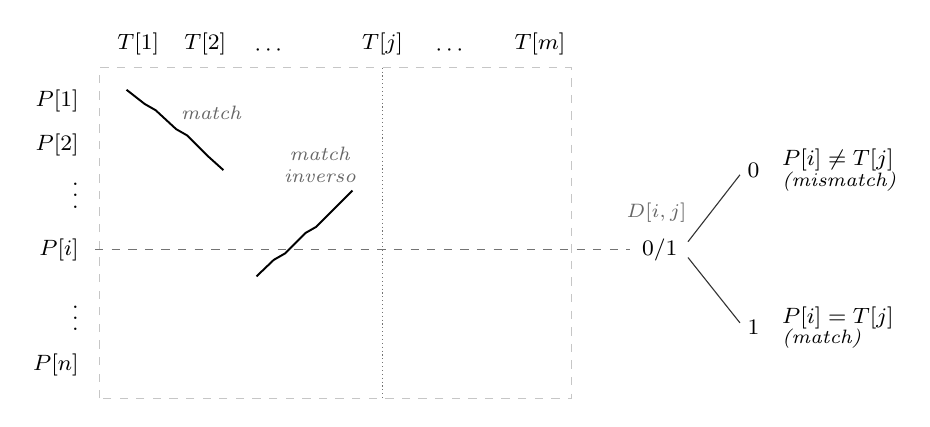
\begin{tikzpicture}[
    x=1cm, y=1cm,
    font=\footnotesize,
    gl/.style={font=\scriptsize, text=black!60, inner sep=1pt},
    et/.style={inner sep=2pt},
  ]

  % --- cornice appena accennata della matrice (nessuna griglia interna) ---
  \draw[gray!45, dashed, line width=0.3pt] (0,0) rectangle (6,4.2);

  % --- colonne: il testo ---
  \node[et, anchor=south] at (0.50,4.28) {$T[1]$};
  \node[et, anchor=south] at (1.35,4.28) {$T[2]$};
  \node[et, anchor=south] at (2.15,4.28) {$\cdots$};
  \node[et, anchor=south] at (3.60,4.28) {$T[j]$};
  \node[et, anchor=south] at (4.45,4.28) {$\cdots$};
  \node[et, anchor=south] at (5.60,4.28) {$T[m]$};

  % --- righe: il pattern ---
  \node[et, anchor=east] at (-0.18,3.78) {$P[1]$};
  \node[et, anchor=east] at (-0.18,3.22) {$P[2]$};
  \node[et, anchor=east] at (-0.18,2.68) {$\vdots$};
  \node[et, anchor=east] at (-0.18,1.89) {$P[i]$};
  \node[et, anchor=east] at (-0.18,1.12) {$\vdots$};
  \node[et, anchor=east] at (-0.18,0.42) {$P[n]$};

  % --- le due linee che individuano la cella (i,j) ---
  \draw[black!55, densely dotted] (3.60,4.20) -- (3.60,0);
  \draw[black!55, dashed]        (-0.05,1.89) -- (6.75,1.89);

  % --- tratto diagonale discendente: allineamento diretto ---
  \draw[line width=0.7pt]
       (0.35,3.92) -- (0.58,3.74) -- (0.72,3.66) -- (0.98,3.42)
    -- (1.12,3.34) -- (1.38,3.08) -- (1.58,2.90);
  \node[gl, anchor=south west] at (1.00,3.50) {\emph{match}};

  % --- tratto antidiagonale ascendente: allineamento invertito ---
  \draw[line width=0.7pt]
       (2.00,1.55) -- (2.22,1.76) -- (2.36,1.84) -- (2.62,2.10)
    -- (2.76,2.18) -- (3.02,2.44) -- (3.22,2.64);
  \node[gl, anchor=south east, align=center] at (3.32,2.70)
       {\emph{match}\\\emph{inverso}};

  % --- valore della cella e biforcazione 0/1 ---
  \node[et, anchor=west] at (6.82,1.89) {$0/1$};
  \node[gl, anchor=south] at (7.08,2.20) {$D[i,j]$};

  \draw[black!80] (7.48,1.99) -- (8.14,2.84);
  \draw[black!80] (7.48,1.79) -- (8.14,0.96);

  \node[et, anchor=west] at (8.16,2.90) {$0$};
  \node[et, anchor=west] at (8.16,0.90) {$1$};

  \node[et, anchor=west, align=left] at (8.60,2.90)
       {$P[i]\neq T[j]$\\[-2pt] {\scriptsize\itshape (mismatch)}};
  \node[et, anchor=west, align=left] at (8.60,0.90)
       {$P[i]=T[j]$\\[-2pt] {\scriptsize\itshape (match)}};

\end{tikzpicture}

\caption{La matrice di bit (\emph{dot-plot}) di $P$ contro $T$: righe indicizzate dal pattern,
colonne dal testo. La cella $(i,j)$ vale $1$ se e solo se $P[i]=T[j]$.}
\label{fig:shift-and-dotplot}
\end{figure}

\begin{osservazione}
Il dot-plot è l'oggetto con cui, in bioinformatica, si confrontano a occhio due sequenze: un
tratto \emph{diagonale} di $1$ --- che scende verso destra --- segnala un match fra un fattore di
$P$ e un fattore di $T$, mentre un tratto \emph{antidiagonale} --- che sale verso destra ---
segnala un match \emph{invertito}, cioè un match fra un fattore di $P$ e un fattore di $T$ letto
al contrario.
\end{osservazione}

Costruire la matrice per intero costa
\[
  \text{tempo per costruirla}\;\longrightarrow\;\Oh(n\cdot m),
  \qquad
  \text{spazio occupato}\;\longrightarrow\;\Oh(n\cdot m)\ \text{bit}.
\]

\begin{dubbio}
Accanto alla parola «bit», sottolineata, il quaderno riporta un'annotazione marginale di una o
due parole che non è stato possibile decifrare.
\end{dubbio}

E allora: questa matrice serve davvero a fare \emph{pattern matching}? Sì, ma non così com'è. Il
punto è che non occorre tenere in memoria un'intera matrice: basta muoversi \emph{per colonne},
un carattere di testo alla volta.

\begin{figure}[H]
\centering
% Il vettore di stato letto per colonne: dall'array al tempo j a quello al tempo j+1
% bastano uno SHIFT (gli 1 scendono di una posizione) e un AND con la maschera.
% ATTENZIONE: le colonne disegnate sono quelle della matrice M dello Shift--And,
% non del dot-plot D (per D la colonna j e' semplicemente la maschera U_{T[j]}).
\begin{tikzpicture}[
    x=1cm, y=1cm,
    font=\footnotesize,
    gl/.style={font=\scriptsize, text=black!60, inner sep=1pt},
    fr/.style={-{Stealth[length=4pt,width=3pt]}, black!70, line width=0.5pt},
  ]

  % --- la matrice, che non viene mai costruita per intero ---
  \draw[black!75] (0,0) rectangle (8.6,5);

  % --- etichette di orientamento (aggiunte per leggibilita') ---
  \node[gl, anchor=south west] at (0.05,5.05) {$T[1]$};
  \node[gl, anchor=south east] at (8.55,5.05) {$T[m]$};
  \node[gl, anchor=east] at (-0.10,4.72) {$P[1]$};
  \node[gl, anchor=east] at (-0.10,0.28) {$P[n]$};

  % --- le due colonne adiacenti j e j+1 ---
  \draw[black!75] (3.30,0) -- (3.30,5);
  \draw[black!75] (3.85,0) -- (3.85,5);
  \draw[black!75] (4.40,0) -- (4.40,5);

  % --- frecce dall'alto: chi sono le due strisce ---
  \draw[fr] (2.55,5.82) to[out=0,in=115] (3.55,5.02);
  \draw[fr] (5.62,5.82) to[out=180,in=65] (4.15,5.02);
  \node[anchor=east, align=center] at (2.45,5.88) {array al\\tempo $j$};
  \node[anchor=west, align=center] at (5.72,5.88) {array al\\tempo $j+1$};

  % --- l'1 scende di una posizione passando da j a j+1 ---
  \node[inner sep=1pt] at (3.575,2.80) {$1$};
  \draw[black!60, densely dotted, -{Stealth[length=3.5pt,width=2.5pt]}]
        (3.575,2.58) -- (3.575,2.28);
  \node[inner sep=1pt] at (4.125,2.42) {$1$};

  % --- un 1 sull'ultima riga: occorrenza completa di P ---
  \node[inner sep=1pt] at (6.00,0.32) {$1$};
  \node[gl, anchor=west] at (6.25,0.32) {occorrenza di $P$};

  % --- le due operazioni ---
  \draw[fr] (2.98,-0.70) to[out=0,in=250] (3.52,-0.05);
  \draw[fr] (4.78,-0.70) to[out=180,in=290] (4.20,-0.05);
  \node[anchor=east] at (2.90,-0.76) {\textsc{shift}};
  \node[anchor=west] at (4.86,-0.76) {\textsc{and}};

\end{tikzpicture}

\caption{Dall'array al tempo $j$ all'array al tempo $j+1$: uno \textsc{shift} verso il basso, che
fa scendere di una posizione gli $1$ già accesi, seguito da un \textsc{and}. L'$1$ disegnato
sull'ultima riga corrisponde a un'occorrenza del pattern. Le colonne disegnate sono quelle della
matrice $M$ della Sezione~\ref{sec:shift-and-matrice}, non del dot-plot $D$.}
\label{fig:shift-and-colonne}
\end{figure}

Ogni colonna del dot-plot è un array di $n$ bit, uno per ciascuna posizione del pattern, e non
costa nulla ottenerla: la colonna $j$ dipende dal solo carattere $T[j]$. Non è però questa la
colonna che conviene far evolvere --- in $D$ un $1$ dice soltanto che due singoli caratteri
coincidono, non che un'occorrenza del pattern è arrivata fin lì. Quello che l'algoritmo tiene in
vita è un unico array di $n$ bit che riassume lo stato dell'intera ricerca: la colonna della
matrice $M$ che definiremo nella Sezione~\ref{sec:shift-and-matrice}. Per passare dall'array al
tempo $j$ a quello al tempo $j+1$ bastano allora due operazioni bit a bit: uno \textsc{shift},
che fa scendere di una posizione tutti gli $1$ già accesi, e un \textsc{and} con una maschera che
dipende dal carattere di testo appena letto --- la maschera della
Definizione~\ref{def:shift-and-maschere}. Un $1$ che arrivi fino all'ultima riga segnalerà
un'occorrenza di $P$ in $T$.


\section{Le maschere del pattern}

\scan{30}
Il pattern è «assimilabile» a una sequenza di $n$ bit, e questo suggerisce di precalcolare, una
volta per tutte, dove ciascun carattere dell'alfabeto compare in $P$.

\begin{definizione}[Maschere del pattern]
\label{def:shift-and-maschere}
Per ogni carattere $x\in\alfa$ si definisce il vettore di bit $U_x\in\set{0,1}^n$ ponendo
\[
  U_x[i]\;=\;
  \begin{cases}
    1 & \text{se } P[i]=x,\\[2pt]
    0 & \text{altrimenti,}
  \end{cases}
  \qquad i=1,\dots,n .
\]
\end{definizione}

La tabella $\set{U_x}_{x\in\alfa}$ mi dice \emph{quale} carattere occorre in $P[i]$: fissata la
posizione $i$, c'è un solo $x$ per cui $U_x[i]=1$, ed è $x=P[i]$. Le maschere si costruiscono una
volta per tutte in preprocessing, a partire dal solo pattern, e occupano $\abs{\alfa}\cdot n$ bit.

Uso allora $\vec{P}$ (il pattern visto come vettore di bit), $T[j]$ e le maschere $U_x[i]$ per
determinare tutte le occorrenze di $P$ in $T$ \emph{senza} costruire il dot-plot: la $j$-esima
colonna del dot-plot è esattamente $U_{T[j]}$, quindi è già precalcolata e la matrice $D$ non va
mai materializzata.


\section{La matrice dello Shift--And}
\label{sec:shift-and-matrice}

Consideriamo ora la matrice $M$ dello Shift--And, matrice che \emph{non} costruiamo per intero ma
che ci permette di risolvere il problema:
\[
  M[i,j]=1 \iff \pre{P}{i}\ \text{è un suffisso di}\ \pre{T}{j},
  \qquad 0\le i\le n,\quad 0\le j\le m ,
\]
con la convenzione $\pre{P}{0}=\vuota$: la riga $i=0$ è allora identicamente $1$ --- la stringa
vuota è suffisso di ogni $\pre{T}{j}$ --- e la colonna $j=0$ è nulla dalla riga $1$ in giù.
Detto altrimenti, $M[i,j]=1$ se e solo se c'è un'occorrenza del prefisso $\pre{P}{i}$ che termina
esattamente in posizione $j$; in particolare gli $1$ dell'ultima riga, quelli con $i=n$, sono
tutte e sole le occorrenze complete di $P$ in $T$. Attenzione a non confondere $M$ con il
dot-plot $D$: dove entrambe sono definite, cioè per $i,j\ge 1$, da $M[i,j]=1$ segue in
particolare $P[i]=T[j]$, quindi $M\le D$ componente per componente, ma non vale il viceversa.

Le condizioni per scrivere correttamente un $1$ in $M[i,j]$ sono due:
\begin{itemize}
  \item[a)] devo avere un $1$ in $M[i-1,\,j-1]$ \quad$\longrightarrow$\quad \textsc{shift};
  \item[b)] deve essere $P[i]=T[j]$ \quad$\longrightarrow$\quad \textsc{and}.
\end{itemize}
Le due condizioni non sono che la lettura ricorsiva della definizione: una stringa di lunghezza
$i$ è suffisso di $\pre{T}{j}$ se e solo se il suo ultimo carattere è $T[j]$ e il suo prefisso di
lunghezza $i-1$ è suffisso di $\pre{T}{j-1}$.

Lette colonna per colonna --- sia $M_j\in\set{0,1}^n$ la $j$-esima colonna di $M$ ristretta alle
righe $1,\dots,n$, cosicché $M_j[i]=M[i,j]$ per $i=1,\dots,n$ --- le due condizioni diventano due
sole operazioni su vettori di bit:
\begin{itemize}
  \item la (a) chiede, per ogni $i$, il bit di riga $i-1$ della colonna precedente: basta far
    scorrere $M_{j-1}$ di una posizione verso il basso, immettendo in testa (\emph{pad}) un $1$,
    \[ \operatorname{shift}(b_1b_2\cdots b_n)\;=\;1\,b_1b_2\cdots b_{n-1}\,; \]
  \item la (b) chiede, per ogni $i$, che sia $P[i]=T[j]$: è esattamente l'\textsc{and} bit a bit
    con la maschera $U_{T[j]}$.
\end{itemize}
In forma vettoriale la ricorrenza è dunque
\[
  M_j\;=\;\operatorname{shift}\bigl(M_{j-1}\bigr)\ \mathbin{\textsc{and}}\ U_{T[j]},
  \qquad j=1,\dots,m ,
\]
ed è da qui che l'algoritmo prende il nome: \emph{uno} shift e \emph{un} and per ogni carattere
del testo.

\begin{osservazione}
Il $1$ immesso in testa dallo \emph{shift} non è un dettaglio implementativo: è la riga $i=0$ di
$M$, quella che i vettori $M_j$ non contengono e che vale costantemente $1$, cioè il fatto che in
\emph{ogni} posizione del testo può iniziare una nuova occorrenza. Con uno shift che immette $0$
la colonna diventerebbe identicamente nulla e l'algoritmo non troverebbe mai nulla. Per la ragione simmetrica la colonna iniziale è nulla, $M_0=0^n$: nessun prefisso non
vuoto di $P$ è suffisso di $\pre{T}{0}=\vuota$.
\end{osservazione}


\section{L'algoritmo}

\begin{algorithm}[H]
\caption{\textsc{Shift-And}}\label{alg:shift-and}
\begin{algorithmic}[1]
\Require $P[1\,..\,n]$, $T[1\,..\,m]$
\Ensure le posizioni di inizio delle occorrenze di $P$ in $T$
\ForAll{$x\in\alfa$}
  \State $U_x \gets 0^n$
\EndFor
\For{$i \gets 1$ \textbf{to} $n$}
  \State $U_{P[i]}[i] \gets 1$ \Comment{$U_x[i]=1$ sse $P[i]=x$}
\EndFor
\State $M_0 \gets 0^n$
\For{$j \gets 1$ \textbf{to} $m$}
  \State $M_j \gets \operatorname{shift}\bigl(M_{j-1}\bigr) \mathbin{\textsc{and}} U_{T[j]}$
  \If{$M_j[n]=1$}
    \State \textbf{output} $j-n+1$
  \EndIf
\EndFor
\end{algorithmic}
\end{algorithm}

\begin{esempio}
Siano $P=\str{aab}$ (quindi $n=3$) e $T=\str{baab}$ (quindi $m=4$). Scrivendo i vettori di bit
dall'alto in basso, da $P[1]$ a $P[3]$, le maschere sono
\[
  U_{\str{a}}=110,\qquad U_{\str{b}}=001,
\]
e la matrice $M$ è quella della Figura~\ref{fig:shift-and-esempio}. Si parte da $M_0=000$ e:
\[
  \begin{aligned}
    M_1 &= \operatorname{shift}(000)\mathbin{\textsc{and}}U_{\str{b}} = 100\mathbin{\textsc{and}}001 = 000, \\
    M_2 &= \operatorname{shift}(000)\mathbin{\textsc{and}}U_{\str{a}} = 100\mathbin{\textsc{and}}110 = 100, \\
    M_3 &= \operatorname{shift}(100)\mathbin{\textsc{and}}U_{\str{a}} = 110\mathbin{\textsc{and}}110 = 110, \\
    M_4 &= \operatorname{shift}(110)\mathbin{\textsc{and}}U_{\str{b}} = 111\mathbin{\textsc{and}}001 = 001 .
  \end{aligned}
\]
L'unico $1$ dell'ultima riga sta in colonna $j=4$: c'è un'occorrenza di $P$ che termina in $4$ e
comincia in $j-n+1=2$, e infatti $\sub{T}{2}{4}=\str{aab}=P$.
\end{esempio}

\begin{figure}[H]
\centering
% La matrice M dello Shift--And per P = aab e T = baab.
% M[i,j] = 1  sse  P[1..i] e' suffisso di T[1..j].
\begin{tikzpicture}[
    x=1cm, y=1cm,
    font=\small,
    gl/.style={font=\scriptsize, text=black!60, inner sep=1pt},
    dia/.style={black!55, dashed, -{Stealth[length=4pt,width=3pt]}, line width=0.5pt},
  ]

  % --- fondo tenue sull'ultima riga (i = n) ---
  \fill[black!8] (0,-1.5) rectangle (3.75,-2.25);

  % --- griglia 3 x 5 (celle di 0.75 cm) ---
  \draw[gray!55, line width=0.4pt, step=0.75] (0,-2.25) grid (3.75,0);
  % separatore fra la colonna di inizializzazione j=0 e le colonne j>=1
  \draw[black!70, line width=1pt] (0.75,0.02) -- (0.75,-2.27);

  % --- intestazioni di colonna: indice j e carattere T[j] ---
  \node[gl, anchor=south] at (0.375,0.44) {$0$};
  \node[gl, anchor=south] at (1.125,0.44) {$1$};
  \node[gl, anchor=south] at (1.875,0.44) {$2$};
  \node[gl, anchor=south] at (2.625,0.44) {$3$};
  \node[gl, anchor=south] at (3.375,0.44) {$4$};

  \node[gl, anchor=south] at (0.375,0.06) {$M_0$};
  \node[anchor=south, inner sep=1pt] at (1.125,0.06) {\texttt{b}};
  \node[anchor=south, inner sep=1pt] at (1.875,0.06) {\texttt{a}};
  \node[anchor=south, inner sep=1pt] at (2.625,0.06) {\texttt{a}};
  \node[anchor=south, inner sep=1pt] at (3.375,0.06) {\texttt{b}};

  % --- intestazioni delle due colonnine di sinistra ---
  \node[gl, anchor=south] at (-1.05,0.06) {$i$};
  \node[gl, anchor=south] at (-0.42,0.06) {$P[i]$};

  % --- etichette di riga: indice i e carattere P[i] ---
  \node[gl] at (-1.05,-0.375) {$1$};
  \node[gl] at (-1.05,-1.125) {$2$};
  \node[gl] at (-1.05,-1.875) {$3$};
  \node[inner sep=1pt] at (-0.42,-0.375) {\texttt{a}};
  \node[inner sep=1pt] at (-0.42,-1.125) {\texttt{a}};
  \node[inner sep=1pt] at (-0.42,-1.875) {\texttt{b}};

  % --- contenuto della matrice ---
  % riga i=1
  \node at (0.375,-0.375) {$0$};
  \node at (1.125,-0.375) {$0$};
  \node at (1.875,-0.375) {$1$};
  \node at (2.625,-0.375) {$1$};
  \node at (3.375,-0.375) {$0$};
  % riga i=2
  \node at (0.375,-1.125) {$0$};
  \node at (1.125,-1.125) {$0$};
  \node at (1.875,-1.125) {$0$};
  \node at (2.625,-1.125) {$1$};
  \node at (3.375,-1.125) {$0$};
  % riga i=3
  \node at (0.375,-1.875) {$0$};
  \node at (1.125,-1.875) {$0$};
  \node at (1.875,-1.875) {$0$};
  \node at (2.625,-1.875) {$0$};
  \node at (3.375,-1.875) {$1$};

  % --- propagazione in diagonale del prefisso che cresce (lo shift) ---
  \draw[dia] (2.05,-0.55) -- (2.45,-0.95)
     node[pos=0.5, sloped, above=3pt, fill=white, inner sep=1pt,
          font=\scriptsize\itshape, text=black!60] {shift};
  \draw[dia] (2.80,-1.30) -- (3.13,-1.63);

  % --- l'ultima riga: gli 1 qui sono occorrenze ---
  \draw[decorate, decoration={brace, amplitude=4pt}, black!60]
        (3.85,-1.5) -- (3.85,-2.25);
  \node[gl, anchor=west, align=left] at (4.18,-1.875)
       {riga $n$: gli $1$ qui\\sono occorrenze di $P$};

  % --- l'occorrenza trovata ---
  \draw[accentdark, line width=0.9pt] (3.375,-1.875) circle (0.29);
  \draw[accentdark, -{Stealth[length=4pt,width=3pt]}, line width=0.5pt]
        (3.55,-2.14) to[out=300,in=170] (4.30,-2.82);
  \node[anchor=west, align=left, font=\scriptsize, text=accentdark] at (4.38,-2.82)
       {occorrenza: $\sub{T}{2}{4}=\str{aab}=P$,\\inizio in $j-n+1=2$};

  % --- maschere applicate colonna per colonna ---
  \node[gl, anchor=north] at (1.125,-2.36) {$U_{\str{b}}$};
  \node[gl, anchor=north] at (1.875,-2.36) {$U_{\str{a}}$};
  \node[gl, anchor=north] at (2.625,-2.36) {$U_{\str{a}}$};
  \node[gl, anchor=north] at (3.375,-2.36) {$U_{\str{b}}$};

  % --- promemoria delle maschere ---
  \node[gl, anchor=north west, align=left] at (-1.20,-2.50)
       {$U_{\str{a}}=110$\\$U_{\str{b}}=001$};

\end{tikzpicture}

\caption{La matrice $M$ dello Shift--And per $P=\str{aab}$ e $T=\str{baab}$. Ogni colonna si
ottiene dalla precedente con uno \emph{shift} (che immette un $1$ in testa) seguito da un
\textsc{and} con la maschera del carattere letto; l'unico $1$ dell'ultima riga segnala
l'occorrenza $\sub{T}{2}{4}=P$.}
\label{fig:shift-and-esempio}
\end{figure}


\section{Complessità}

\[
  \Oh(n\cdot m)\ \text{tempo},\qquad \Oh(n)\ \text{bit di spazio (\emph{working space})} .
\]

\begin{osservazione}
La stima $\Oh(n\cdot m)$ è una \emph{sovrastima}: conta le celle di $M$, che però non viene mai
costruita. Il ciclo esegue $m$ iterazioni, ciascuna con \emph{uno} shift e \emph{un} and su
vettori di $n$ bit; nel modello word-RAM con parola di $w$ bit il costo della ricerca è
\[
  \Th\!\left(m\left\lceil \frac{n}{w}\right\rceil\right),
\]
che vale $\Th(m)$ non appena $n\le w$, cioè quando il pattern ha «una lunghezza ragionevole»
(a margine, a matita, una nota in gran parte illeggibile richiama proprio questo:
\lacunainl{\dots\ \str{/64}\ \dots}, la parola di macchina da $64$ bit).
Analogamente, lo spazio $\Oh(n)$ bit è quello della sola colonna corrente $M_j$: va aggiunta la
tabella delle maschere, $\abs{\alfa}\cdot n$ bit, trascurabile per alfabeti di dimensione
costante. Il testo viene letto in \emph{streaming}, un carattere alla volta.
\end{osservazione}


\section{Variazioni sul tema}

Lo Shift--And è la prima delle due variazioni sul tema del pattern matching annunciate dopo
Karp--Rabin: quella che sfrutta il parallelismo della parola di macchina, impacchettando in una
stringa di bit lo stato dell'intera ricerca e facendolo avanzare con una sola istruzione di shift
e una sola di and. La seconda variazione è la \emph{ricerca approssimata}, cioè il pattern con
errori: non viene sviluppata qui e sarà ripresa più avanti, con le nozioni di distanza e di
allineamento. L'estensione bit-parallela naturale in quella direzione consiste nel mantenere
$k+1$ vettori invece di uno --- uno per ogni numero di errori ammessi da $0$ a $k$ --- ed è la
famiglia Shift-Add / Wu--Manber.
